\picturechapter{Cross-ID: Analysis and visualization of complex XL−MS-driven
  protein interaction networks}{Chaptercovers/ch2.pdf} \label{ch-2}
\vspace*{0.25cm}

{\footnotesize Sebastiaan C. de Graaf\textsuperscript{*}, Oleg Klykov\textsuperscript{*}, Henk van den Toorn, and Richard A. Scheltema}

\begin{center}
  \vspace{3cm}
  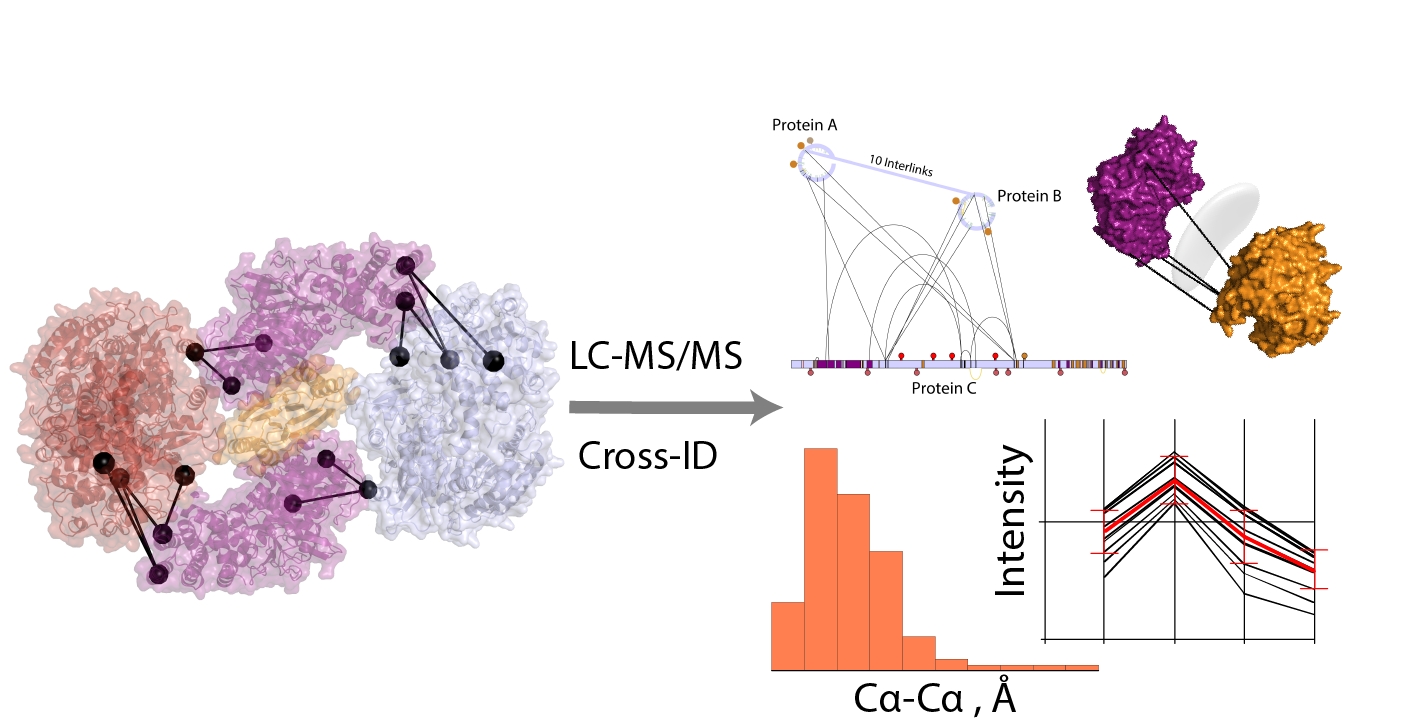
\includegraphics[]{Chapter.2/Figures/ch2.png}
  \vspace{0.25cm}
\end{center}

\begin{flushleft}
  \vspace*{\fill}
  \rule{\textwidth}{1pt}\\[0cm]
  \textbf{This chapter is based on work in the following publication:}\\
  \footnotesize{
    \textbf{Cross-ID: Analysis and Visualization of Complex XL−MS-Driven
      Protein Interaction Networks, \emph{Journal of Proteome Research}} (2019), 18:642-651, doi:10.1021/acs.jproteome.8b00725\\
    %%\footnotesize
    \vspace{0.3cm}
    \textsuperscript{*} These authors contributed equally to this work}
\end{flushleft}

\begin{abstract102}
  Protein interactions enable much more complex behavior than the sum of the individual protein parts would suggest and represents a level of biological complexity requiring full understanding when unravelling cellular processes. Crosslinking mass spectrometry has emerged as an attractive approach to study these interactions and recent advances in mass spectrometry and data analysis software have enabled the identification of thousands of crosslinks from a single experiment. The resulting data complexity is however difficult to understand and requires interactive software tools. Even though solutions are available, these represent an agglomerate of possibilities and each features its own input format often forcing manual conversion. Here we present Cross-ID, a visualization platform that links directly into the output of XlinkX for Proteome Discoverer, but also plays well with other platforms by supporting a user-controllable text-file importer. The platform includes features like grouping, spectral viewer, GO enrichment, PTM-visualization, domain- and secondary structure mapping, dataset comparison, pre-visualization overlap-check and more. Validation of detected crosslinks is available for proteins and complexes with known structure or for protein complexes through the DisVis online platform. Graphs are exportable in PDF format, and datasets can be exported in tab separated text files for evaluation through other software.
\end{abstract102}
\thumbforchapter

\section{Introduction}
\lettrine[lraise=0.1, nindent=0em, slope=-.5em]{P}{rotein}
interactions represent a level of cellular complexity that is essential for almost all biological processes. The protein assemblies they represent are highly dynamic and orchestrate cellular processes by regulating enzymes and forming macromolecular clusters capable of more complex behavior than the sum of their parts would suggest. Crosslinking mass spectrometry (XL-MS) has emerged as an attractive approach to elucidate protein-protein interactions (PPIs) by mass spectrometry. It uses small reagents with two reactive moieties capable of forging a covalent bond between two amino acids in close proximity. Upon application to proteins and protein-protein complexes followed by their proteolytic digestion, four distinct peptide products are formed: non-modified, mono-linked, loop-linked, and crosslinked peptides \cite{schilling2003ms}. The first three product groups consist of single peptides in various forms that yield limited or no structural information. The fourth group consists of two peptides captured by the crosslinking reagent; this yields valuable distance information for the elucidation of protein tertiary structure (the two peptides originate from the same protein) or protein quaternary structure (the two peptides originate from different proteins). Identification of both peptides by mass spectrometry allows for localization of the crosslink within the proteins of interest. Although several well established methods like affinity purification mass spectrometry (AP-MS) \cite{fagerlund2017spacer, benda2014structural, joachimiak2014structural, herzog2012structural, chen2010architecture, armony2016cross-linking} are available for studying PPIs at high speeds \cite{hosp2015double-barrel}, most of these are limited to stable interactions and/or provide little to no structural information. XL-MS on the other hand has the potential to capture weak and transient interactions complete with structural information. With recent advances in mass spectrometry, crosslinker chemistry, pre-fractionation techniques and data analysis software, XL-MS can now routinely detect thousands of crosslinked peptides from a single experiment \cite{kao2011development, liu2015proteome-wide, liu2017optimized, schweppe2017mitochondrial}. Even in the case of single proteins, XL-MS can yield hundreds of detected distance restraints \cite{belsom2017complementary}.
\begin{figure*}[!htb]
  \center
  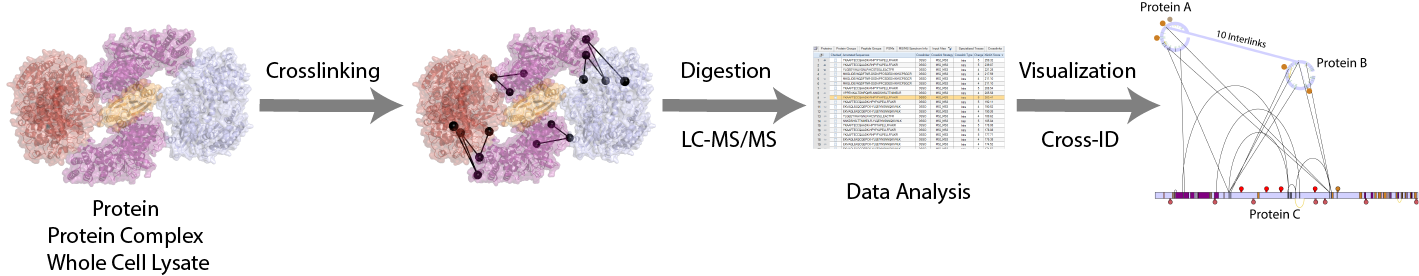
\includegraphics[]{Chapter.2/Figures/f1.png}
  \captionsetup{singlelinecheck = false, format= hang}
  \caption{\textbf{Visualization with Cross-ID.}}
  \label{fig:fig2.1}
\end{figure*}

\begin{figure*}[!htb]
  \center
  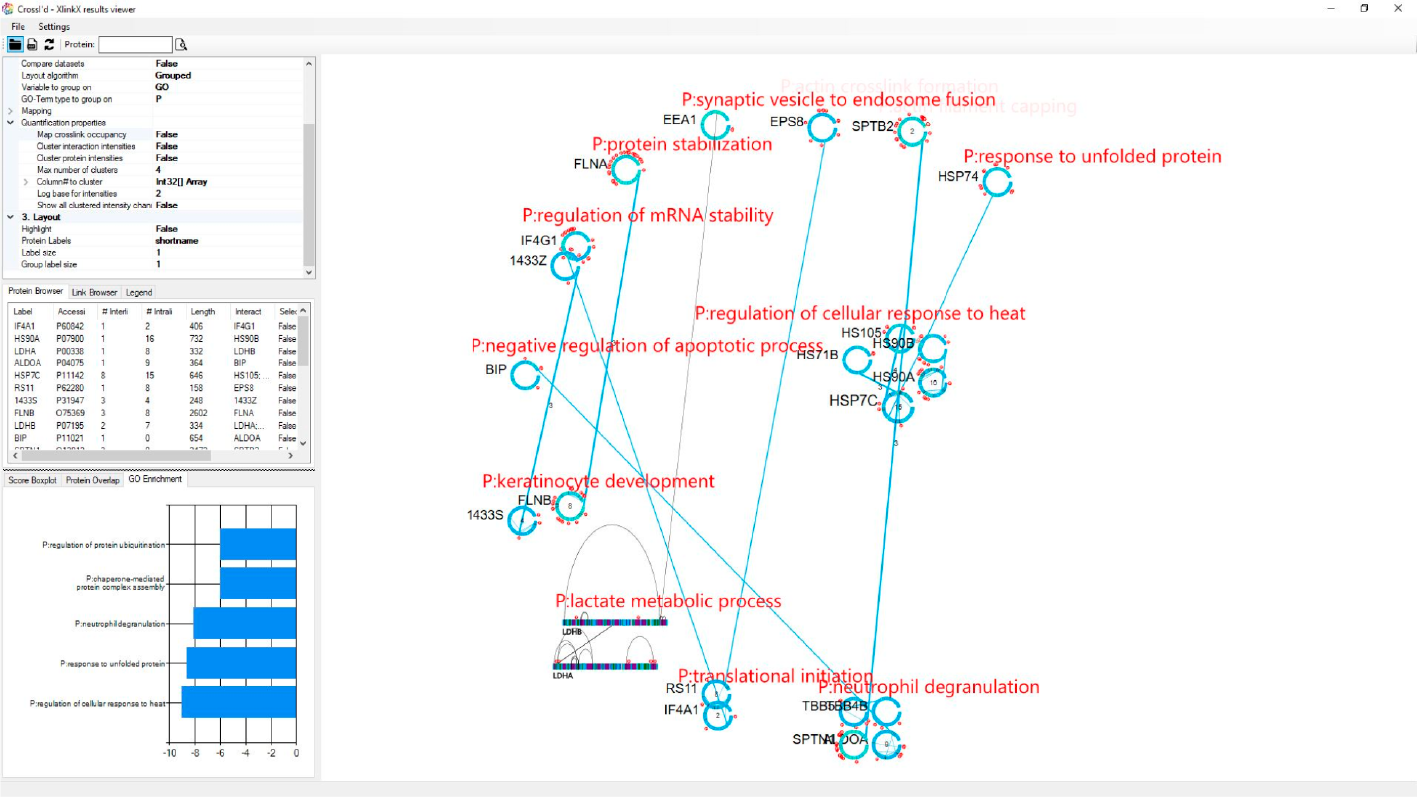
\includegraphics[]{Chapter.2/Figures/f2.png}
  \captionsetup{singlelinecheck = false, format= hang}
  \caption{\textbf{Screenshot of Cross-ID.}}
  \label{fig:fig2.2}
\end{figure*}

An attractive means to obtain a bird’s-eye view of the crosslinking results are network graphs \cite{shannon2003cytoscape:, cline2007integration, bastian2009gephi:}. This type of visualization however also becomes cumbersome to read for increasing sizes of the depicted datasets, where the large number of nodes and edges can easily obfuscate the view \cite{agapito2013visualization}. Additionally, when no connection between the visualized elements and the initial input datasets exists it remains very difficult for the user to browse the data and check for validity. To circumvent these obstacles advanced software allowing the network to be visualized, organized and filtered in real-time is needed. Several software platforms partly supporting such features exist \cite{courcelles2017clmsvault:, heymann2008msx-, kahraman2011xwalk:, kosinski2015xlink, lima2015sim-xl:, riffle2016proxl, schweppe2015xlmap:, schweppe2016xlinkdb, solis-mezarino2017complexview:}, with varying degrees of specificity towards XL-MS. The most widely used examples consist of xiNet \cite{combe2015xinet:} and xVis \cite{grimm2015xvis:}. Each of these tools has a unique set of features and each offers a different subset of visualization options, which tailors them for particular applications (e.g. Xwalk \cite{kahraman2011xwalk:} calculates solvent accessible surface distances or XlinkAnalyzer \cite{kosinski2015xlink} fits distance restraints to a given 3D model). However, when it comes to visualization of large scale crosslinking datasets like whole cell lysates, a combination of software solutions is often required. Proteome-wide interactomes can for example be visualized with biological network builders such as Cytoscape \cite{shannon2003cytoscape:, cline2007integration}, but there are no tools specifically tailored towards in-depth analysis of large proteome-wide XL-MS datasets. Added to this, relatively few tools support generic input formats from multiple software platforms (prominent example which do include this are xiNET \cite{combe2015xinet:} and ProXL \cite{riffle2016proxl} ); however, most are tightly linked to a specific search engine or define their own data format requiring cumbersome file format changes to compare results between different datasets.
Here we present Cross-ID, a standalone solution for visualization of XL-MS data as network graphs. It provides a direct connection to the output of XlinkX for Proteome Discoverer 2.3 but also supports an importer for comma-separated text output generated by any XL-MS search engine. Additional to crosslinking data, Cross-ID can display any data containing connection or distance restrains (e.g. small-angle X-ray scattering or SAXS data \cite{morimoto2013small-angle} ) as long as it is available in a tabular form. The importer uses natural language processing to predict the use of each column-header in the output file and allows the user to make adjustments where required. The generated graphs are highly interactive and can be explored by filtering, expanding, repositioning, highlighting, mapping or altering the graph directly. Ultimately, this will enable the user to draw meaningful conclusions from the graphs edited inside Cross-ID and without the need for editing the input dataset each time before uploading. It is also possible to group proteins based on detected interlinks or according to other parameters (e.g. their GO enrichment coefficient), significantly simplifying the data analysis. A number of site-specific findings from the Uniprot database \cite{bateman2017uniprot:} (among others glycosylation, disulfide bridges and phosphorylation sites) can be mapped onto all protein representations, as well as residues of interest. In addition, it is also possible to depict specific modifications detected by the search engine and quantitation by various methods. Cross-ID also supports validation of crosslinks for a single protein or protein complex using available structures in protein data bank (PDB) format. Alternatively, Cross-ID provides a direct link to DisVis for validating potentially interacting partners based on the detected crosslinks \cite{zundert2016disvis, zundert2015disvis:}. As a showcase study we provide a whole cell lysate dataset with 2754 crosslink spectra matches (CSMs), obtained from PC9 cells. To showcase the quantitation functionalities we used Tandem Mass Tag (TMT) quantitation to quantitate protein kinase A (PKA), activated upon addition of cAMP as a model system.


\section{Materials and Methods}

\subsection{DSSO Protein-Protein Crosslinking}
Crosslinked cell lysates have been prepared as previously described \cite{klykov2018efficient}. Briefly, PC9 (Sigma-Aldrich, Steinheim, DE) cells were collected and washed 3x with PBS (Lonza, Basel, SUI). After centrifugation, the cell pellet was resuspended in crosslinking buffer consisting of 50 mM HEPES, 150 mM NaCl and 1.5 mM MgCl\textsubscript{2} (all from Sigma-Aldrich, Steinheim, DE). Protease inhibitors (Roche, Basel, SUI) and 0.5 mM DTT (Sigma-Aldrich, Steinheim, DE) were added right before use. After the cells were lysed with a Bioruptor (Diagenode SA, Seraing, BE), freshly dissolved disuccinimidyl sulfoxide or DSSO in DMSO (Sigma-Aldrich, Steinheim, DE) was added to a final concentration of 2 mM. The crosslinking reaction was quenched after 30 minutes with Tris-HCl at a final concentration of 20 mM. The crosslinked proteins were denatured and reduced and alkylated in a mixture of 8 M Urea, TCEP and CAA. Proteolytic digestion was performed in 2 steps: for 30 min with LysC (Wako, Tokyo, JPN) at room temperature and overnight with Trypsin (Promega, Madison, WI, USA) at 37 ⁰C. Digested peptides were desalted with a Sep-Pak cartridge and dried prior to fractionation.


\subsection{Fractionation of Crosslinked Peptides}
Strong Cation Exchange (SCX) chromatography was performed on an Agilent 1200 HPLC system (Agilent Technologies, Waldbronn, DE). The setup was previously described \cite{hennrich2011improving}, but shortly consists of an Opti-Lynx trap column connected to a PolyLC SCX-separation column (PolyLC Inc., Columbia, MD, USA). Peptide mixtures were reconstituted in 5\% DMSO/10\% formic acid/85\% water (v/v/v) and separated over a gradient of 120 minutes, resulting in 50 collected factions. A total of 15 crosslinks-rich fractions were chosen for analysis and prior to further analysis dried and stored at -80 ⁰C.


\subsection{LC-MS/MS Analysis}
Peptide mixtures were reconstituted in 5\% DMSO/10\% formic acid/85\% water (v/v/v) and analyzed on an Orbitrap Fusion Lumos (Thermo Fisher Scientific, San Jose, CA, USA) coupled online to an Agilent 1290 UPLC (Agilent Technologies, Waldbronn, DE). Peptides were trapped on a double-frit C\textsubscript{18} pre-column (Reprosil C\textsubscript{18}, Dr. Maisch, 100 µm x 2 cm, 3 µm; packed in-house) for 5 min with buffer A (0.1\% formic acid) and separated on a single-frit analytical column (Poroshell 120 EC C18, Agilent Technologies, 50 µm x 50 cm, 2.7 µm) over 155 minutes with a linear gradient from 10\% to 40\% B (B: 0.1\% formic acid, 80\% acetonitrile). Optimized MS settings were described previously \cite{liu2017optimized, klykov2018efficient}. Acquired data were analyzed with the Proteome Discoverer software suite 2.3 (Thermo Fisher Scientific, San Jose, CA, USA) with incorporated XlinkX nodes. Spectra were matched against the Homo sapiens database from SwissProt (version 2018\_06, 20,349 sequences, downloaded from Uniprot). The protease was set to “Trypsin” and the maximum number of missed cleavages was defined as 2. Carbamidomethylation of cysteines was set as fixed modification and oxidation of methionine and protein N-terminal acetylation as variable modifications. For the linear peptide search, precursor mass tolerance was defined as 20 ppm and fragment mass tolerance as 0.5 Da for ion trap readout or 20 ppm for the Orbitrap readout. For the crosslinked peptides search, the minimum peptide length was set to 5 and minimum peptide mass to 300, while the maximum peptide mass was set to 7000. The precursor mass tolerance was set to 10 ppm, FTMS fragment mass tolerance at 20 ppm and ITMS fragment mass at 0.5 Da. FDR threshold was set to 0.01 (1\%) and FDR strategy as “Percolator”.


\subsection{TMT Experiments}
TMT labels were purchased from Thermo Fisher Scientific (San Jose, CA, USA) and the labelling protocol performed according to supplier instructions after desalting of the crosslinked peptides. 10 channels were used to label 10 samples of model system PKA (Sigma-Aldrich, Steinheim, DE) solubilized at a concentration of 5.74 µM with added cAMP (Sigma-Aldrich, Steinheim, DE) ligand to the final concentration of 0-8 µM and 10 µM respectively. Digestion, fractionation and LC-MS/MS analysis were performed according to the procedure described above, except for alterations to the LC gradient consisting of increasing the starting point from 5\% to 36\% of buffer B. For this data, the Orbitrap Fusion (Thermo Fisher Scientific, San Jose, CA, USA) with tune page version 3.1.2412.14 was used for data acquisition with the standard template for TMT labeled crosslinking samples. For data analysis, the TMT-specific nodes were added to the standard crosslinking data acquisition protocol \cite{klykov2018efficient} after “Precursor Ion Exclusion” node namely: “Isobaric Tag Loss” was set to TMT, “Precursor Selection Range” with Mass Range 400-1200 \emph{m/z} followed by 10 SPS scans with HCD at 65\% NCE and resolution of 50000 in Orbitrap. Recorded data were searched against PKA protein complex proteins with 200 Human proteins as decoys taken from the reviewed Swiss-Prot database. In addition to the standard XlinkX processing workflow, “Reporter Ions Quantifier” node was added with “Integration Tolerance” set to 0.03 Da and “Centroid With Smallest Delta Mass” as “Integration Method”. For the consensus workflow, “Reporter Ions Quantified” node was included with standard settings.
\begin{figure*}[!htb]
  \center
  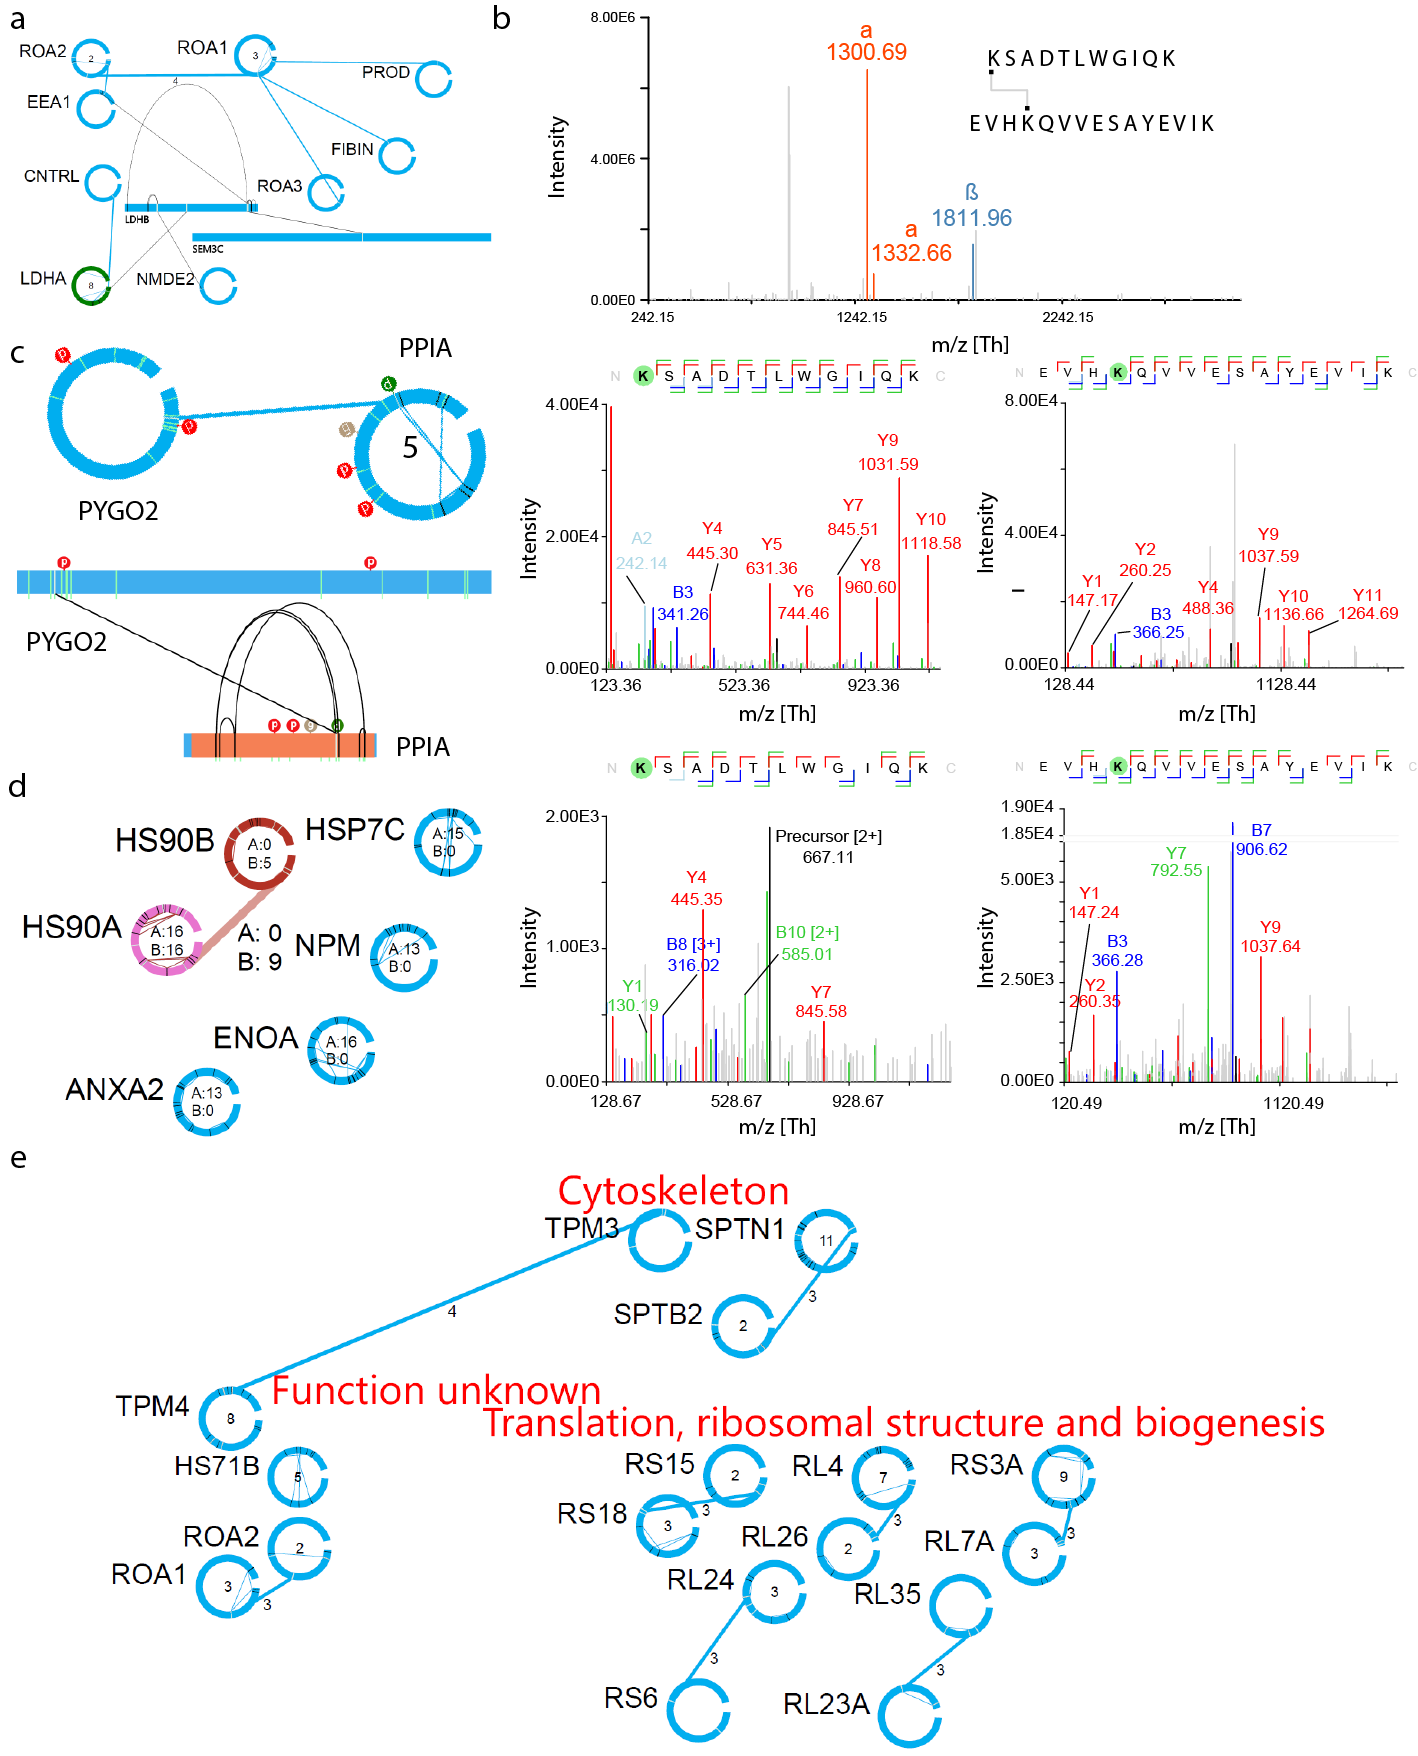
\includegraphics[]{Chapter.2/Figures/f3.png}
  \caption{
    \textbf{Visualization with Cross-ID on a PC9 whole proteome data set.} ~~a) Snapshot of the generated protein interaction network. ~~b) Spectral viewer for selected top-scored cross-links. ~~c) Comparison of bar and circle views for filtered proteins with depicted phosphorylation, glycosylation, and DSSO monolinks together with the known protein domain. ~~d) Comparison of cross-links filtered by XlinkX score at 50 with 13 intralinks and 7 interlinks. ~~e) Clustering according to the EggNOGG database for filtered proteins.
  }
  \label{fig:fig2.3}
\end{figure*}


\subsection{Software and Data Availability}
Cross-ID was developed in Microsoft Visual Studio 2017 as a C\# WinForms application using Windows Presentation Foundation elements. The GraphX .NET library was used as the foundation for the network visualizations. For running the tool, minimally .NET version 4.7 needs to be installed. The software can be downloaded from https://www.hecklab.com/software/xlinkx/ together with an instruction video. The raw data, all the associated output and databases used in this study have been deposited to the Proteome-Xchange Consortium \cite{vizcaíno2014proteomexchange} via the PRIDE partner repository with the identifier PXD008418 (already published and openly accessible) for the whole-proteome dataset and PXD011077 (user: reviewer59676@ebi.ac.uk; password: 7H5TMR0l) for the TMT dataset.
\begin{figure*}[!htb]
  \center
  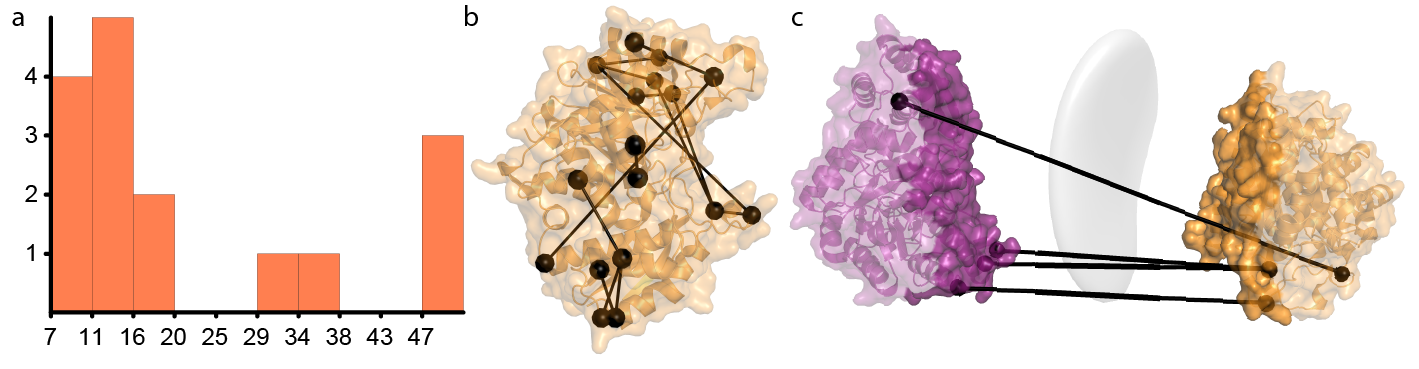
\includegraphics[]{Chapter.2/Figures/f4.png}
  \caption{
    \textbf{Validation of cross-links detected for alpha-enolase.} ~~a) Distance distribution of mapped cross-links on alpha-enolase. ~~b) Detected crosslinks on crystal structure. ~~c) Interaction interface generated by DisVis based on indicated restraints (grey surface) in comparison to the existing dimeric interface (dark purple and dark orange).
  }
  \label{fig:fig2.4}
\end{figure*}
\begin{table*}[!htb]
  \center
  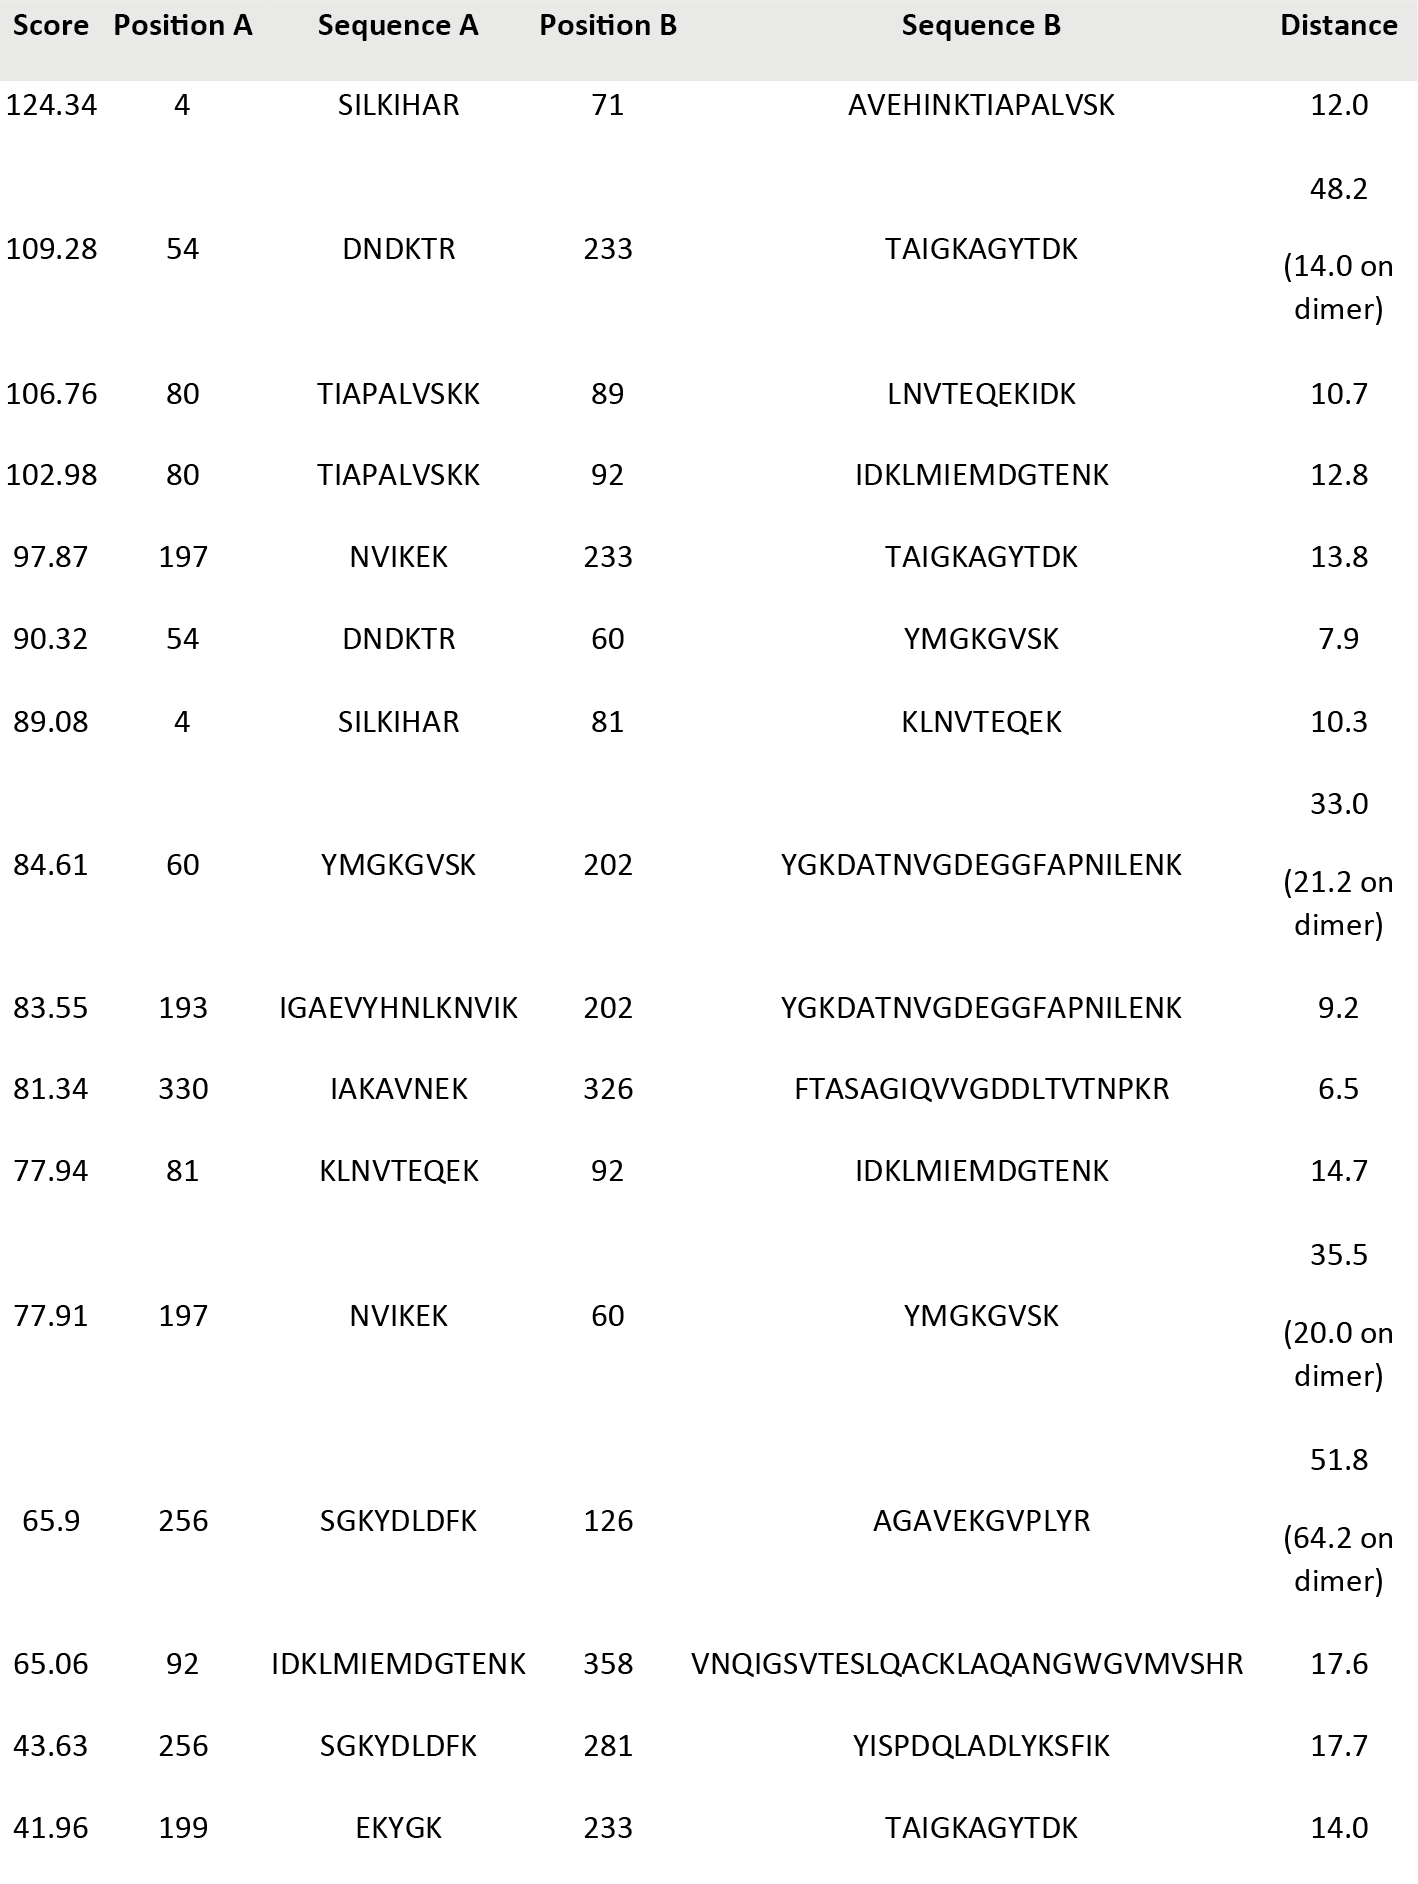
\includegraphics[]{Chapter.2/Figures/t1.png}
  \captionsetup{singlelinecheck = false, format= hang}
  \caption{
    \textbf{List of Crosslinks Detected for Alpha-Enolase.}\\
  }
  \label{tab:tab2.1}
\end{table*}

\section{Results and Discussion}

\subsection{Data Import}
Cross-ID provides a direct link to the output generated by the XlinkX nodes integrated in the Proteome Discoverer data analysis environment \cite{klykov2018efficient}. The files with extension ‘.pdResult’ contain all information required to build the visualization of the network, including the spectra and protein information, together with the tables generated by XlinkX. By loading this directly, correctness and access to all required information is ensured. To work with output from other search engines, Cross-ID provides a convenient import interface for tab- or comma-delimited text files, with column names on the first line. Since column names are not fixed between different search engines, or even in some cases between different versions of the same search engine, Cross-ID assists in manually selecting the correct columns. It provides a prediction of the purpose of each column by calculating a Levenshtein distance \cite{levenstein1966binary} to pre-defined column names.
The full Uniprot database \cite{bateman2017uniprot:} is supported by Cross-ID and is used to provide additional information about the identified proteins, like known PTMs and secondary/tertiary structure information. It can however only do so when the crosslinked peptides contain valid Uniprot accessions from the proteins they derive from (e.g. when the RAW data was analyzed against a protein FASTA file extracted from Uniprot). For those cases where Uniprot accessions are not available, Cross-ID automatically provides the opportunity to load the appropriate protein FASTA file for basic visualization and validation tasks described later.


\subsection{Basic Protein Visualization}
To show the basic functionality of Cross-ID we provide a whole cell lysate dataset with 2754 CSMs, obtained from PC9 cells (\textbf{\autoref{tab:tabdummy2.1}}). Individual proteins are visualized either as a horizontal bar or circular view, with the addition of their short or full protein name or the Uniprot accession number in the form of an editable label. For a ‘clean’ view these labels can be removed completely or resized. At any time the visualization style can be altered from circular to bar or vice-versa by mouse right-click for each individual protein (\textbf{\autoref{fig:fig2.2}a}). Both the circular and horizontal bar protein visualizations represent the amino acid sequence in clockwise fashion or from left to right respectively. In the horizontal bar, the width of the bar represents the length of the amino acid sequence, helping to get insight in the relative sizes of the different proteins and the exact positions of the detected crosslinks. To provide initial insight in the potential of PTM-driven interactions, both representations can be annotated with PTMs visualized as spherical tags containing the first letter describing the modification, both from Uniprot and/or detected by the search engine. Uniquely for the circular view, grey lines on the circle depict residues involved in interlinks. Interlinks are connected by a line between circles, at the positions from the crosslink with the highest score. The number of crosslinks between two proteins is shown above the connecting line, something which is also reflected by the thickness of the line. Black lines on the circle depict residues involved in intralinks, which are also connected by a line inside the circle. A number inside the circle depicts amount of unique intralinks. To assist in locating proteins with a high degree of interconnectivity, the size of both the circular display and the label are scaled according to the amount of interlinks detected for that protein. In addition, switching from circular to the horizontal bar view, provides insight into both domain and secondary structure information extracted from Uniprot.
Using a search bar, individual proteins and crosslinks can easily be located within the graphs by full name, abbreviated name or accession. All proteins involved in crosslinks are displayed in the protein browser tab and detected crosslinks in the link browser. Here the user can center the graph on selected proteins/crosslinks, sort and filter based on the source dataset, number of inter- or intra-links, associated GO-term (when grouped by GO-term) and whether or not the protein has been selected. Browsers can be sorted on a column by clicking the column name, while clicking the right mouse button on column names opens a filtering menu. For example, in the link browser, interactions can be filtered and sorted through both protein names (“source” and “target”), the number of crosslinks representing the interaction, the maximum score, dataset origin and crosslink type by mouse clicking on these column names. The protein browser can be filtered and sorted in a similar manner. To assess the data underlying the visualization, both the proteins and connecting lines can be clicked to access a list of all associated crosslinks and their properties. Selecting an individual crosslink in this list provides another list of associated CSMs and selecting a CSM shows the associated spectra in an integrated spectrum viewer together with information about the linked peptides and all detected modifications (\textbf{\autoref{fig:fig2.2}b}). This option will however only work when the path to the folder containing the (Thermo) raw file has been correctly specified.


\subsection{Graph Visualization Options}
The network graph can be laid out in three different fashions: circular layout, Lin Log layout \cite{noack2007energy} or via one of various grouping options. The Lin Log algorithm positions the largest groups of interconnected nodes in the center of the graph, and places groups of interconnected nodes increasingly further from the center the smaller they are, thereby minimizing the “energy” of the graph \cite{pajntar1900overview}. The grouping algorithm can group on GO-terms, source dataset, by protein function according to the eggNOGG database \cite{huerta-cepas2016eggnog}, by creating hubs of equally interconnected proteins or by user-defined groups (\textbf{\autoref{fig:fig2.2}e}). In all cases, the largest group of proteins is placed at the center as a circle of nodes and the rest of the groups as smaller circles around it. The GO-term grouping is determined by comparing the frequency of the associated terms to either occurrence in a reference dataset (provided in the form of a list of accession numbers) or in the whole genome of the organism under investigation by performing a Fisher’s Exact test \cite{rivals2007enrichment}. The term with the lowest resulting \emph{p}-value for each type of GO-term chosen by user (“P” for Pathway, “F” for Function or “C” for Compartment) is assigned as the term of interest for a given protein, and grouping can be done based on a term of interest for any of these three types. When clustered by connectivity, proteins are localized according to the number of interacting partners providing interaction hubs.
To make the graph more clear, crosslinks and/or proteins can be hidden through several mechanisms. For example, display of inter- and/or intra-links can be turned off and a minimum score can hide potentially lower quality crosslink identifications. Alternatively, displayed proteins can be filtered based on the minimum number of inter- or intralinks (\textbf{\autoref{fig:fig2.2}c}). Within the link or protein browser more intricate filters can be assembled as well (right-click the column of interest, select filtering and implement the desired filter). The filtered datasets, as displayed in the protein browser or link browser, can consequently be exported as a .CSV file and if required loaded again into Cross-ID, enabling the creation of more compact graphs. Cross-ID also implements functionality to easily compare two datasets (e.g. controls vs experimental groups). When comparing multiple datasets, proteins and interactions are colored based on which dataset they occur in: dataset 1 – darkred, dataset 2 – blue, or both – pink (\textbf{\autoref{fig:fig2.2}d}). Additionally, the number of crosslinks from each dataset is provided and a filter responsive Venn-diagram is included as well, indicating overlap for shown proteins. To support replicates, there is an overlap-check function for multiple datasets which requires as additional input a minimum number of datasets in which a crosslink must occur before it is included in the final dataset. Additionally, the fraction of crosslinks included in the final dataset is shown, as well as a Venn-diagram if more than one input file was provided. As before, the filtered dataset can be exported to .CSV or directly used as a dataset for further processing.


\subsection{Mapping Detected Crosslinks to Existing Structures}
An often time-consuming task when analyzing crosslinking data is mapping the detected crosslinks on existing structures. A major hurdle here is that the sequences in structures in PDB format tend to not precisely match those in standard databases like Uniprot, usually caused by truncations, point mutations or exclusive availability of a structure from another organism. Such differences require a lot of time-consuming and error-prone manual work to locate the correct position for each crosslink. Especially for large structures like the ribosome, this task quickly becomes infeasible. Automation is therefore desirable and a number of separate solutions are available. One of the notable examples is Xlink Analyzer \cite{kosinski2015xlink}, a Chimera \cite{pettersen2004ucsf} module which requires only structure and distance restraints as an input for mapping. Similar input information is required for the R package XLmap \cite{schweppe2015xlmap:}, which also generates overlaid plots of crosslinked sites on contact maps and assigns a score to each model. Cross-ID incorporates extensive automation for this cumbersome task. It aligns the sequences used for analysis and those encapsulated within the crystal structure file using the Smith-Waterman local sequence alignment together with the BLOSUM62 substitution matrix \cite{henikoff1992amino}. Non-natural amino acids such as pyrrolysine and selenocysteine are automatically substituted with standard lysine and cysteine respectively prior to alignment. The minimum sequence similarity for this step can be defined by the user, but is set by default to 60\% which works well in most cases. This initial alignment step is used to determine which proteins’ structure is represented in the provided PDB structure and select these proteins and their crosslinks as candidates for validation. Next, alignment of the selected crosslinks’ peptides by the same protocol is performed. Again a minimum sequence similarity can be defined, but the default is 88\%. To guide the process the residues involved in the crosslink can be defined, set by default to lysine. In case another residue is matched after alignment, the software automatically verifies whether this residue is characterized by similar chemistry (e.g. arginine instead of lysine). In those cases where this is not so, the crosslink is flagged and the user can decide on a case-to-case basis how to proceed. Afterwards, the crosslink positions are mapped to the structure, and Euclidian distances between the Cα atoms of linked residues are calculated and presented in a filter-responsive list. This list also contains the last 8 characters of the PDB filename and the detected distances, as well as amino acid sequences of crosslinked peptides with the highest sequence overlap. Upon completion, the user is presented with a dialog summarizing the validation by detailing the amount of unvalidated intra and inter-links, substituted residues and flagged residues. The distribution of the found distances is automatically shown in a histogram (\textbf{\autoref{fig:fig2.3}a}).
Another major hurdle is the preparation of the existing structures and crosslinking data for automated docking procedures. Cross-ID also provides far-reaching automation for these purposes by integrating with the DisVis/HADDOCK computational structural docking environment \cite{dominguez2003haddock:, zundert2016haddock, zundert2015disvis:, zundert2016disvis}. For this purpose, Cross-ID currently provides automated access to DisVis \cite{zundert2016disvis, zundert2015disvis:}, although we intend to add more options in future releases. Given a known structure for potential interacting partners, DisVis is able to predict prospective interaction interfaces based on user-supplied distance restraints (\textbf{\autoref{fig:fig2.3}c}), and has already been applied successfully to XL-MS datasets \cite{klykov2018efficient}. Restraints which are violated in the predicted interface will be marked as false positives and will be omitted prior to further modelling steps. A score indicating the probability of occurrence of each of the restraints between the submitted structures is calculated as well. All required files are automatically prepared and uploaded based on the results from the sequence alignment step described above. Prior to upload, the minimum and maximum restraint length can be changed manually. As a model for validation we used alpha enolase, which has a known PDB structure (PDB ID: 2PSN; resolution 2.2 Å). For this protein, XlinkX detected a total of 28 crosslinks (\textbf{\autoref{tab:tabs2.1}}) of which 16 are on enolase alone (\textbf{\autoref{tab:tab2.1}}). Of these, 12 restraints are within the DSSO crosslinking distance of 30 Å while four exceed this (\textbf{\autoref{fig:fig2.3}b}). Enolase however exists in solution as a dimer, meaning that the violated restraints are potentially crosslinks between the two subunits. To verify this, we submitted chain A and chain B from a known PDB structure with only the outliers to DisVis (\textbf{\autoref{tab:tabs2.2}}). Three out of four restraints were detected as valid and indeed could be mapped on a dimer structure with distances of 14.0 Å, 20.0 Å and 21.2 Å. The remaining restraint has been detected by DisVis as a false-positive and can be mapped on a dimer with a distance of 64.2 Å (\textbf{\autoref{tab:tabs2.3}}).


\subsection{Quantitation}
Quantitation of crosslinks is rapidly becoming an important facet for crosslinking analyses, providing insight in structural rearrangement of proteins upon stimulation. To support quantitation coming from crosslink analysis, Cross-ID offers two quantitation parameters in the generated graphs: intensities and crosslink occupancy (representing how often a pair of residues were actually crosslinked as opposed to not modified or mono-linked). The latter value is mapped as a heat-colored circle on the crosslink line (black for 0, white for 1 and a scale from red to yellow in between). In case intensities are provided, the column names in the input file have to be edited accordingly (\textbf{\autoref{tab:tab2.2}}). Measured CSM intensities (from label-free or labeling experiments like TMT) are clustered using the k-means algorithm \cite{jain1900data}. When several identified spectra for the same crosslink positions are quantified, the median value is taken for further analysis. The number of clusters is set by default to 4. The clustered intensities are subsequently visualized in table format within the graph, using heat colored squares, the color of which is determined by their log transformed intensity relative to the rest of the cluster. The number of columns of this table can be set to match the number of clustered intensity channels. The intensity values are automatically log transformed before clustering and the base of this log transformation can be set by the user. Within the table representation, a column represents the experiment (e.g. in the case of TMT labeling, the first column represents channel 1, etc.). The clustered values can be accessed for a more detailed overview by pressing the “C” key while clicking on either the edge (for interaction clustering) or the protein (for protein intensity clustering). The crosslinks sorted by cluster are returned, as well as a line graph for the selected cluster showing the median intensities as a thick red line with error bars and all the individual intensities as faded out gray thin lines.
\begin{table*}[!htb]
  \center
  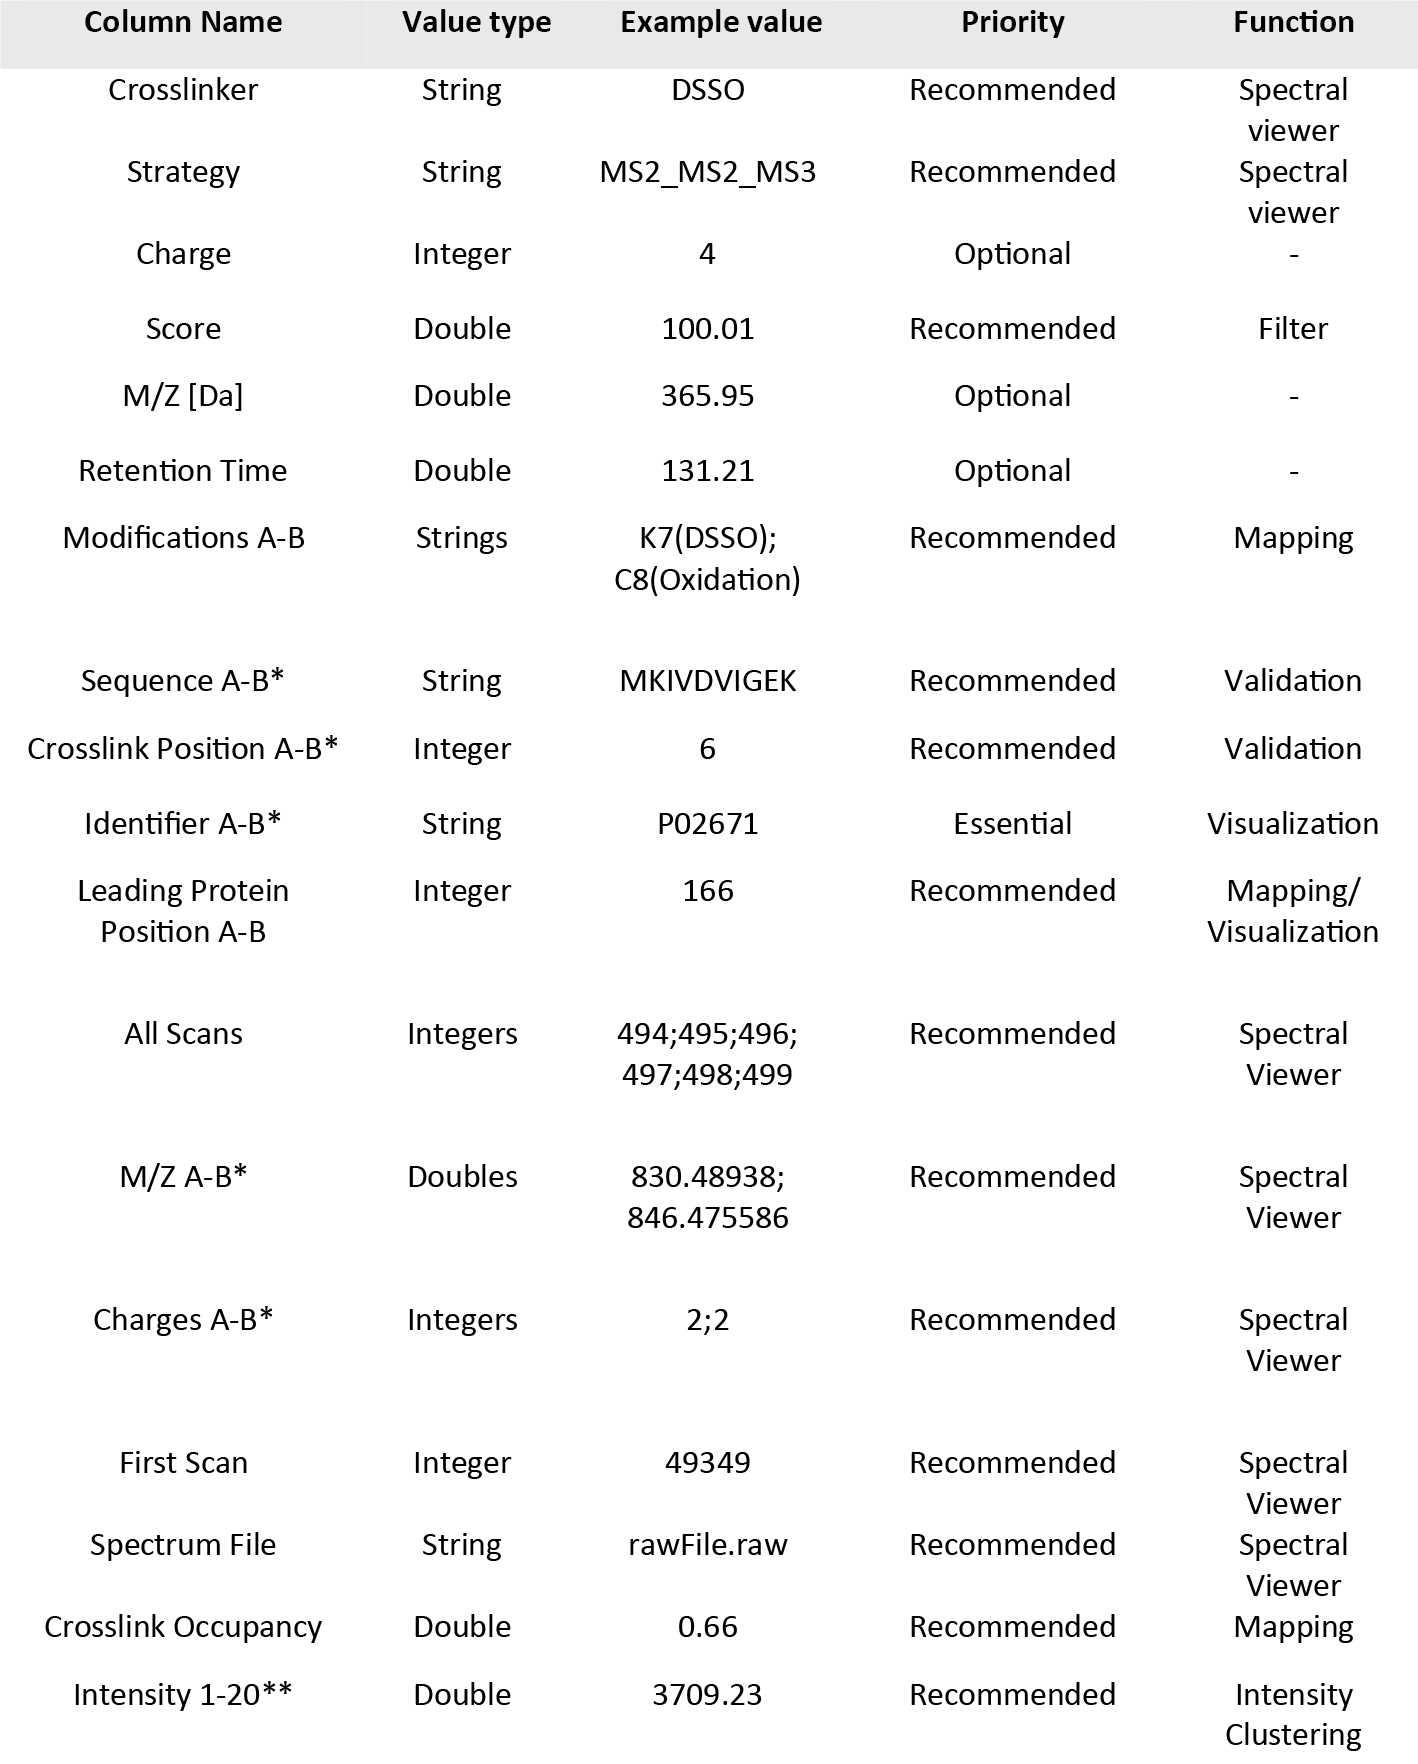
\includegraphics[]{Chapter.2/Figures/t2.png}
  \caption{
    \textbf{Recommended Input Format for Cross-ID}\textsuperscript{a}\\
    \textsuperscript{a}Optional columns were kept for the purpose of providing the user with additional information for inspection in tabular format and for exporting.\\
    \textsuperscript{b}Columns with a name indicating a range (e.g., charges A−B) indicate multiple columns with the same requirements. Columns needing an array of values (e.g., “all scans”) require those values to be separated by semicolons.\\
    \textsuperscript{c}Intensity columns are imported through a separate mechanism to avoid cluttering of the importer form. This means that the intensity columns should be named: intensity1, intensity2, and so on. Other column names do not require specific formatting as long as the importer is used.
  }
  \label{tab:tab2.2}
\end{table*}

To demonstrate the ability of Cross-ID to rapidly leverage quantitation information, we performed TMT labelling experiments on the bovine Protein Kinase A (PKA) complex. PKA is a tetramer composed of two regulatory subunits and two catalytic subunits. Each regulatory subunit is able to bind 2 molecules of cyclic AMP (cAMP), upon binding the catalytic subunits are released. We used TMT 10-plex to measure the structural behavior for increasing concentrations of cAMP. There are two types of regulatory subunits; for each type the alpha- and beta-forms are present and a complex can be formed either by combination of the alpha- and beta-forms or by one a single form. Catalytic subunits are also present as alpha- and beta-forms, but only one of the forms is present in the PKA complex. As the structure for the bovine type II alpha regulatory subunit is missing, we modelled this protein from residue 97 to 402 with I-TASSER \cite{yang2014i-tasser} (\textbf{Structure \ref{struct:structdummy2.1}}), using the available template from mouse (PDB ID 3TNP with resolution 2.3 Å, chain ~~b) . As structure with the bound cAMP ligand, we used a previously modelled structure from the SWISS-MODEL repository \cite{bienert2017swiss-model} (\textbf{Structure \ref{struct:structdummy2.2}}). We detect 5 intralinks for the type II regulatory subunit alpha-form (Uniprot accession P00515, \textbf{\autoref{fig:fig2.4}a}) and for the beta-form no crosslinks. The catalytic subunit is represented by the alpha subunit with 5 intralinks (Uniprot accession P00517, \textbf{\autoref{fig:fig2.4}a}). In both cases, it was possible to group the behavior of all detected crosslinks into 4 clusters even though the number of maximum clusters was set to 5 (see \textbf{\autoref{tab:tabdummy2.5}} and \textbf{\autoref{fig:figs2.1}a-d}).It is known that the regulatory subunit undergoes conformational changes upon binding of cAMP. Cluster 3 and 4 contain crosslinks with increasing intensities for increasing concentrations of cAMP. Crosslink 187-269 is mapped as 46.6 Å when no ligand is present (see \textbf{\autoref{fig:fig2.4}b}) and 21.0 Å with the ligand present (see \textbf{\autoref{fig:fig2.4}c}); for this crosslink we detect a 10-fold increase in intensity. Crosslink 342-376 is mapped as 21.2 Å on the holoenzyme regulatory subunit and quantified with relatively low intensity in the control experiment. On the folded conformation the same restraint is 30\% shorter and shows an intensity increase upon cAMP addition of almost 4–fold. There is one unmapped crosslink between lysine residues 315, which is located on the surface exposed flexble loop and might belong to an alternative folded conformation of the complex. Notably, the remaining crosslinks are mapped within the DSSO crosslinking range for at least one of the conformations of the regulatory subunit (\textbf{\autoref{tab:tabdummy2.6}}). The catalytic subunit is released upon cAMP binding and with this release cteayes a highly dynamic protein with domains involved in hinge and shear motions \cite{akamine2003dynamic}. Even though it is expected that this protein is very flexible, all detected intra-links can be mapped on the available apoenzyme structure (PDB ID 5VI9 with resolution 1.9 Å, chain ~~a) within the DSSO maximum crosslinking distance (\textbf{\autoref{tab:tabdummy2.6}}). Crosslink 24-193 is located in cluster 1 (\textbf{\autoref{fig:figs2.1}e}) and shows a drastic decrease in intensity for higher concentrations of cAMP. This behavior is not readily explainable, but we hypothesize that upon substrate binding the protein is made structurally less flexible by formation of a salt-bridge between one of these lysines and Asp’162 (see \textbf{\autoref{fig:fig2.4}d}).
%%TODO caption overflows
\begin{figure*}[!htb]
  \center
  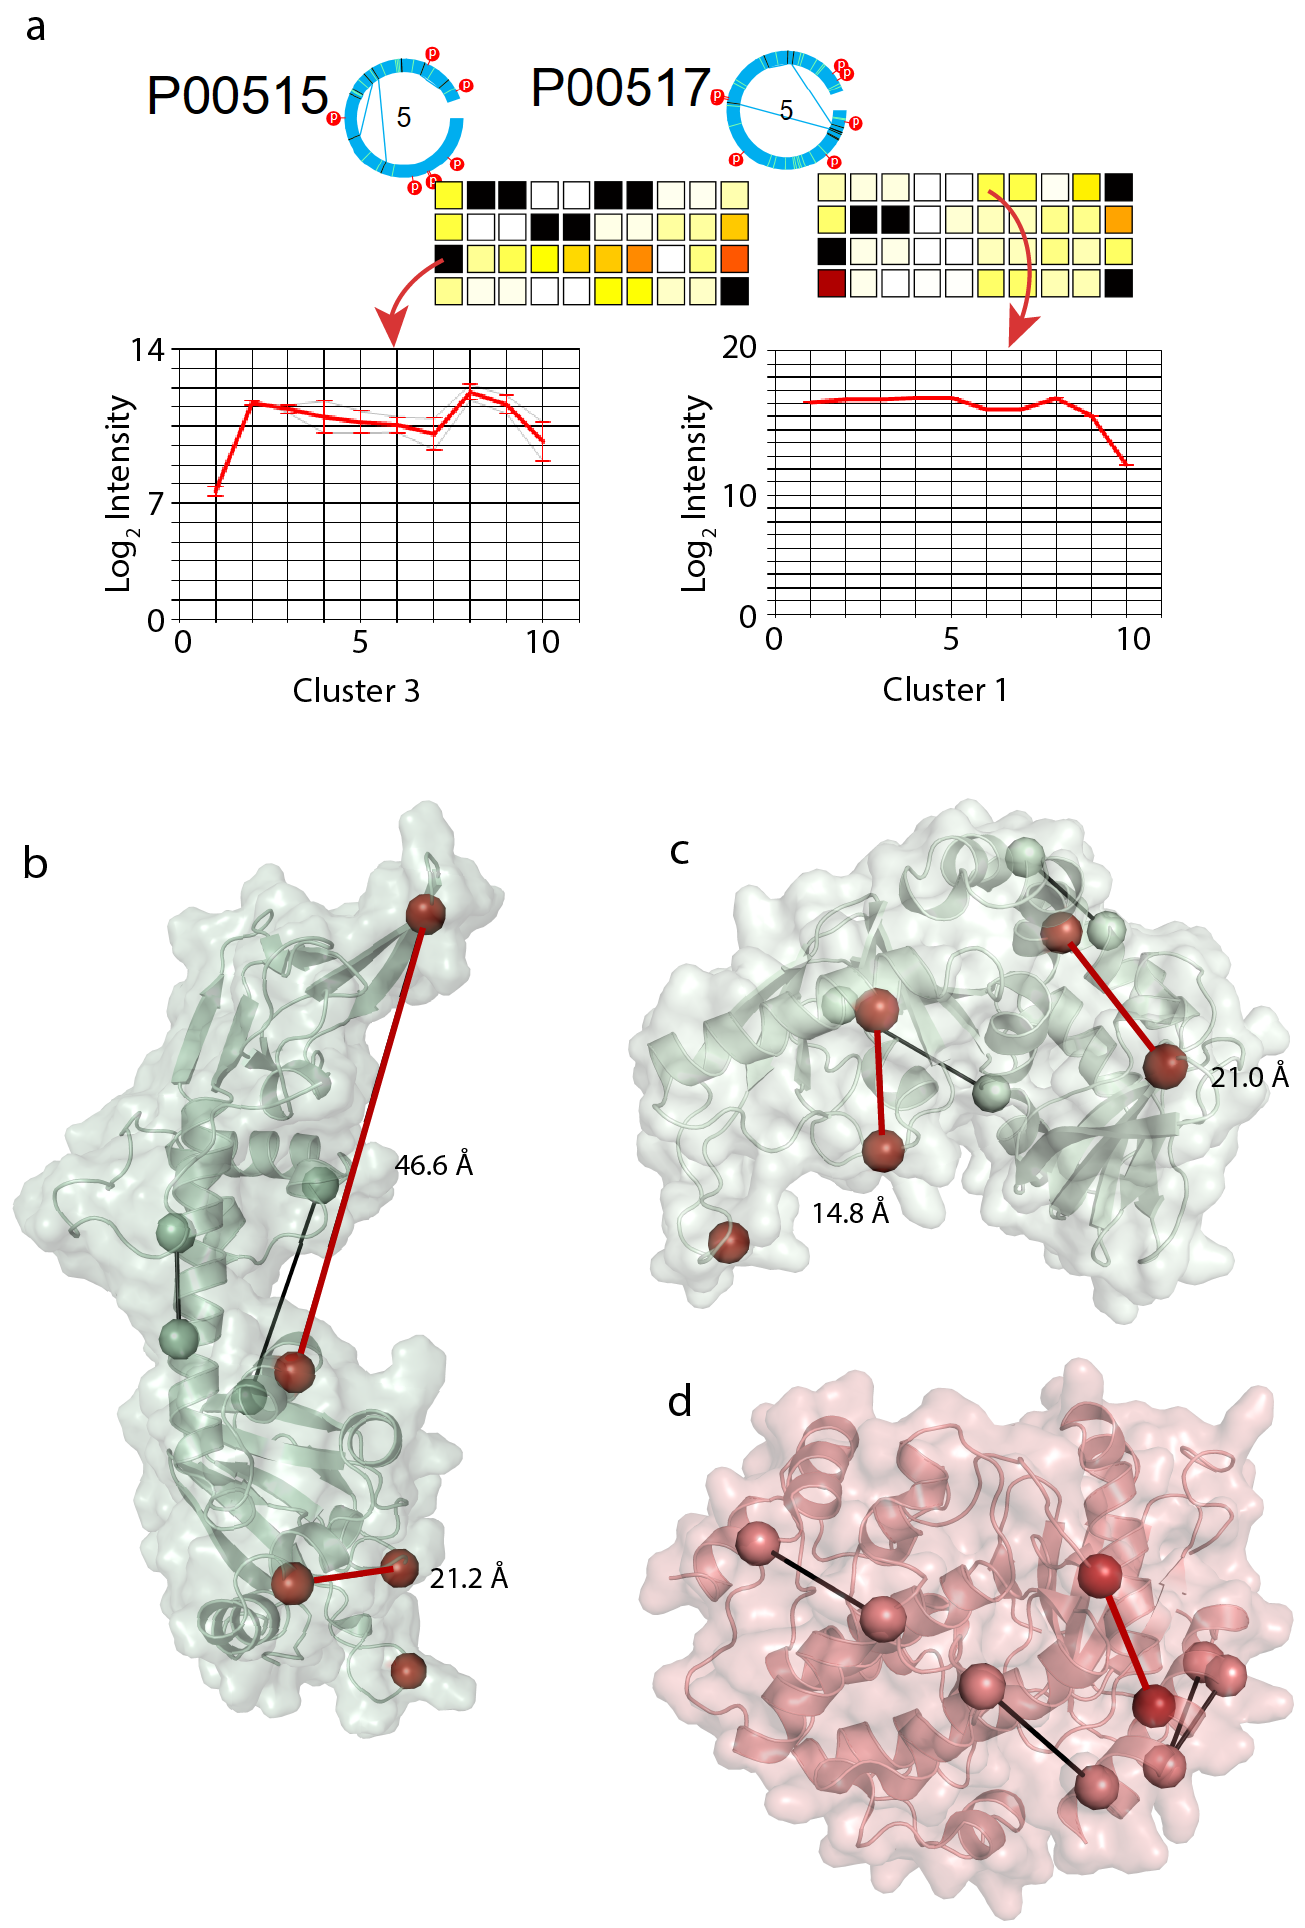
\includegraphics[]{Chapter.2/Figures/f5.png}
  \caption{
    \textbf{Quantitation with Cross-ID.} ~~a) Detected cross-links for the PKA complex in circular representation (left: regulatory subunit; right: catalytic subunit alpha). ~~b) Ligand-free and ~~c) cAMPbounded structures of bovine alpha type II regulatory subunit. ~~d)
    Structure of bovine catalytic subunit alpha with mapped cross-links. Cross-links mapped in black do not change intensity across TMT channels, whereas residues and cross-links mapped in dark red are changing their intensity across the TMT channels.
  }
  \label{fig:fig2.5}
\end{figure*}


\section{Conclusions}
Crosslinking mass spectrometry experiments tend to produce such large amounts of data, that processing rapidly becomes impractical – especially in the case of whole proteome experiments. To alleviate this we present Cross-ID, a tool that produces graph presentations of crosslinking data and offers several tools to bring the detected crosslinking data into structural data like crystal structures. It offers optimal integration with the XlinkX data analysis pipeline \cite{liu2017optimized, klykov2018efficient}, but also supports import of data in CSV format from other search engines with partial automation through a natural language importer. Various forms of grouping of the protein network are supported for gaining optimal insights in the detected data, with support for grouping on external data like e.g. GO annotations. To support analyses of the detected crosslinks on existing crystal structure data, Cross-ID implements automated sequence alignment to bridge the differences between the used sequences and those in the crystal structures. As further support in this direction, it also offers a convenient interface to the structural modeling pipeline of DisVis/HADDOCK. With support for various quantitation options with automated clustering, the tool provides a very detailed look at structures from a crosslinking point-of-view. Cross-ID was developed with extensibility in mind and as part of the XlinkX data analysis pipeline will see continued development and support. Future functionalities currently already under development include: integration of PPI databases such as String \cite{szklarczyk2015string} and CORUM \cite{ruepp2008corum:} to group based on known complexes, further integration with the HADDOCK software for structural modelling, implementation of true distance measures like e.g. Xwalk implements \cite{kahraman2011xwalk:}, integration with standardization efforts like mzIdentMl, and many others. To further integrate with other softwares, we aim to add support for non csv/text based output formats like pepXML \cite{hoopmann2016open} and/or pepXMLTab \cite{xiaojingwang2018pepxmltab:}.

\subsection{Acknowledgements}
We thank all Heck-group members for their helpful contributions and enduring early testing. From the Bonvin-lab we thank Alexandre Bonvin and Jörg Schaarschmidt for integration with the DisVis platform. From Thermo Fisher Scientific we thank Bernard Delanghe, Kai Fitzemeier and Frank Berg for their collaboration on incorporating the XLinkX crosslink search engine into the Proteome Discoverer software and Rosa Viner for her collaborative work on DSSO crosslinking and support in mass spectrometry method development. We acknowledge financial support by the large-scale proteomics facility Proteins@Work (Project 184.032.201) embedded in the Netherlands Proteomics Centre and supported by the Netherlands Organization for Scientific Research (NWO). Additional support came through the European Union Horizon 2020 program FET-OPEN project MSmed (Project 686547), and the European Union Horizon 2020 program INFRAIA project Epic-XS (Project 823839).

\subsection{Author contributions}
R.A.S. conceived of the study. O.K. performed the XL-MS experiments and provided ideas for features. S.C.d.G., H.v.d.T., and R.A.S. programmed Cross-ID. S.C.d.G., O.K. and R.A.S. wrote the paper, whereafter all authors critically read and edited the manuscript.

\clearpage
\begin{subappendices}
  \beginsupplement

  \section{Supplementary material}
  Supplementary Structure 1-2, Supplementary Result 1-2 and Supplementary Table 1 and 5-6 can be found online at:\\
  \emph{https://pubs.acs.org/doi/full/10.1021/acs.jproteome.8b00725}\\
  The Cross-ID software, documentation and instructional video can be found online at:\\
  \emph{https://www.hecklab.com/software/xlinkx}\\
  \refstepcounter{table}
  \label{struct:structdummy2.1}
  \refstepcounter{table}
  \label{struct:structdummy2.2}
  \addtocounter{table}{-2}
  \refstepcounter{table}
  \label{tab:tabdummy2.1}
  \addtocounter{table}{3}
  \refstepcounter{table}
  \label{tab:tabdummy2.5}
  \refstepcounter{table}
  \label{tab:tabdummy2.6}
  \addtocounter{table}{-6}

  \begin{figure*}[!hbt]
    \center
    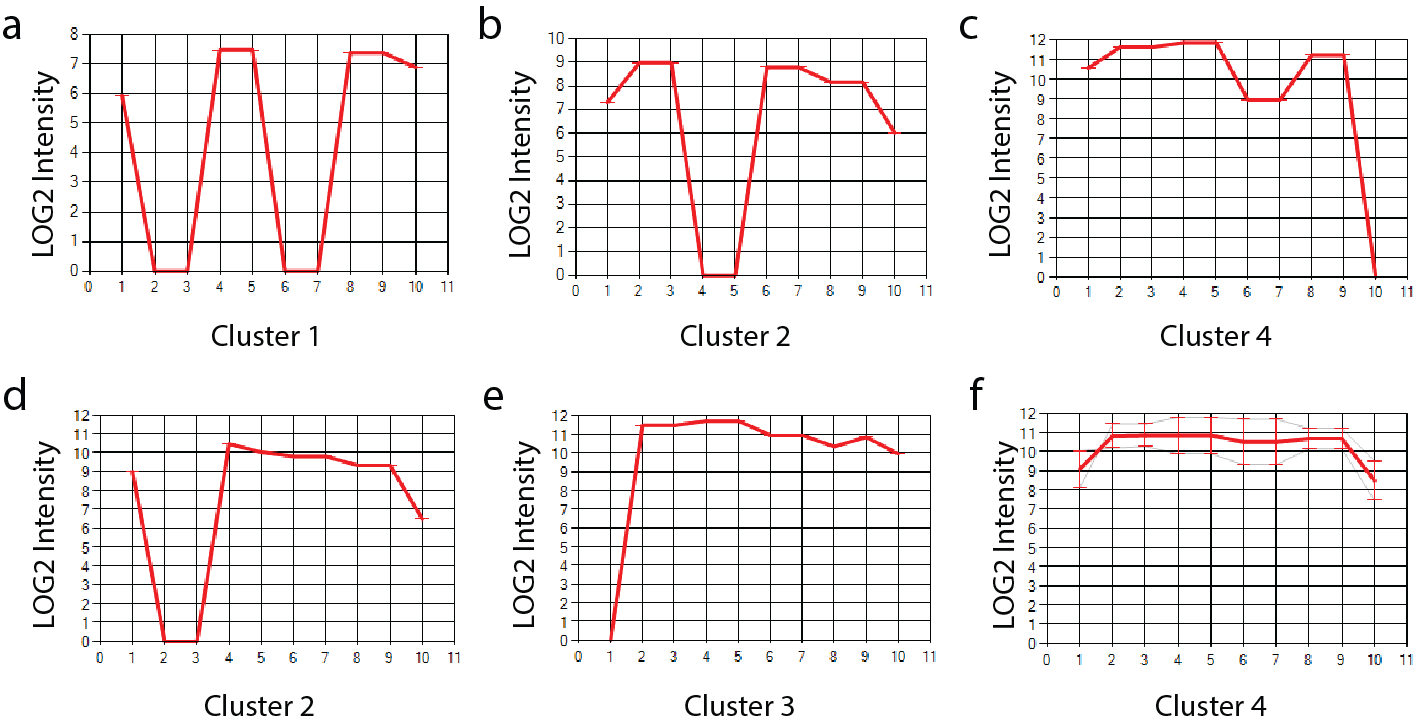
\includegraphics[]{Chapter.2/Figures/fs1.png}
    \caption{
      \textbf{Intensity clusters generated with Cross-ID for TMT-labelled crosslinked peptides of Protein Kinase A proteins.} TMT channels 1 to 10 corresponds to increasing concentration of cAMP ligand from 0 µM for channel 1 and 10 µM for channel 10. (A-D) Crosslinks intensity for bovine type II regulatory subunit alpha. (E-F) Crosslinks intensity for bovine catalytic subunit alpha.
    }
    \label{fig:figs2.1}
  \end{figure*}
  \vspace{1cm}
  \begin{table*}[!hbt]
    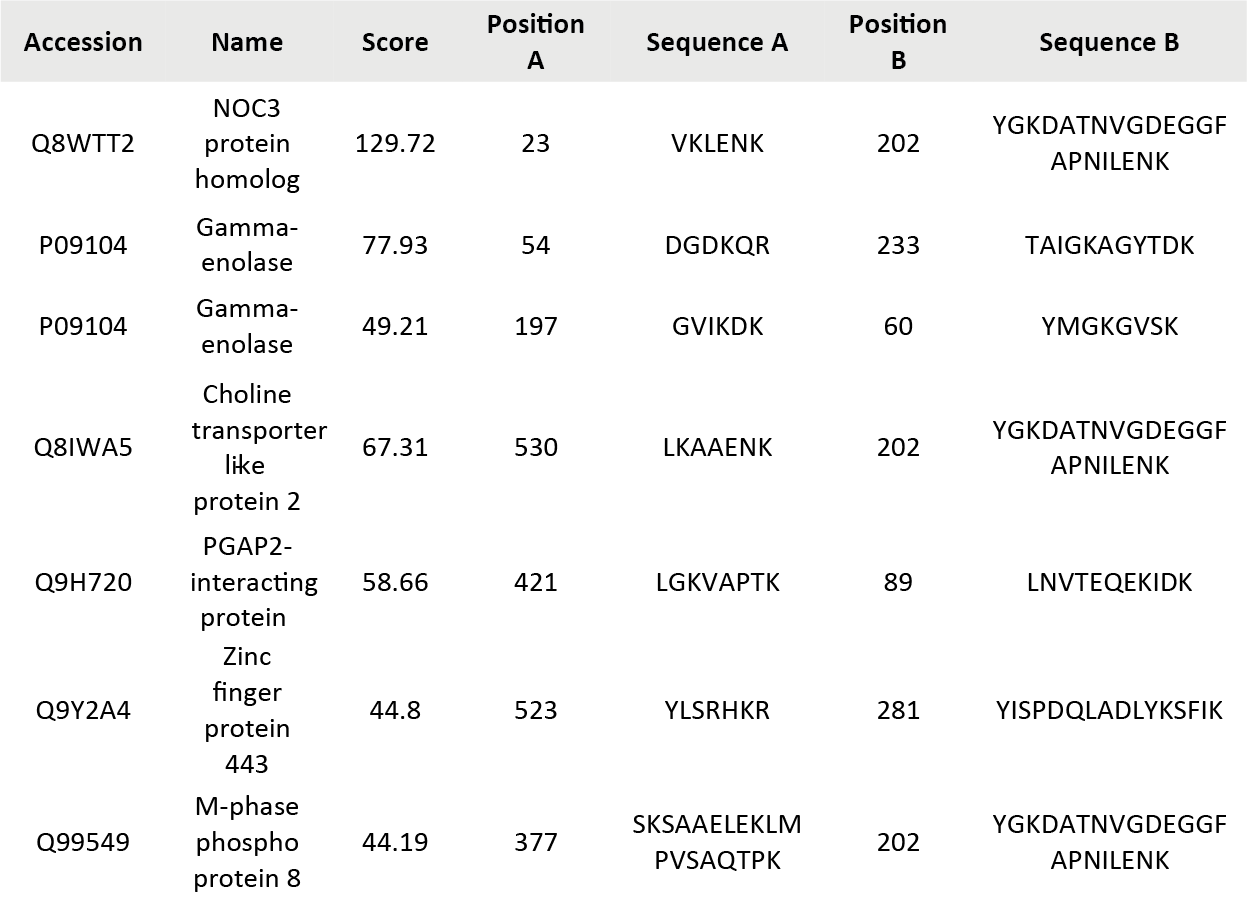
\includegraphics[]{Chapter.2/Figures/ts1.png}
    \captionsetup{singlelinecheck = false, format= hang}
    \caption{
      \textbf{Detected and mapped interlink-crosslinks for Alpha-Enolase.}
    }
    \label{tab:tabs2.1}
  \end{table*}
  \vspace{1cm}
  \begin{table*}[!hbt]
    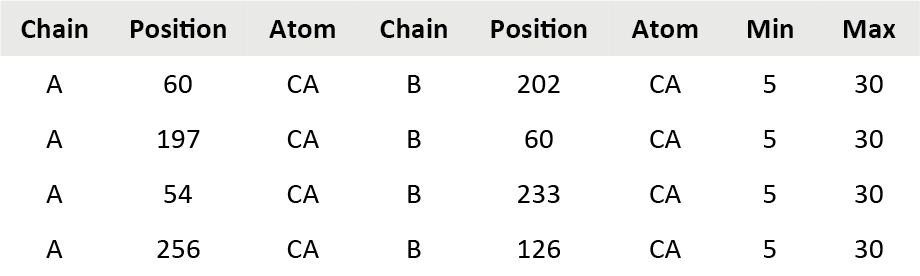
\includegraphics[]{Chapter.2/Figures/ts2.png}
    \captionsetup{singlelinecheck = false, format= hang}
    \caption{
      \textbf{DisVis input example file for potentially intersubunit Alpha-Enolase crosslinks.}
    }
    \label{tab:tabs2.2}
  \end{table*}
  \vspace{1cm}
  \begin{table*}[!hbt]
    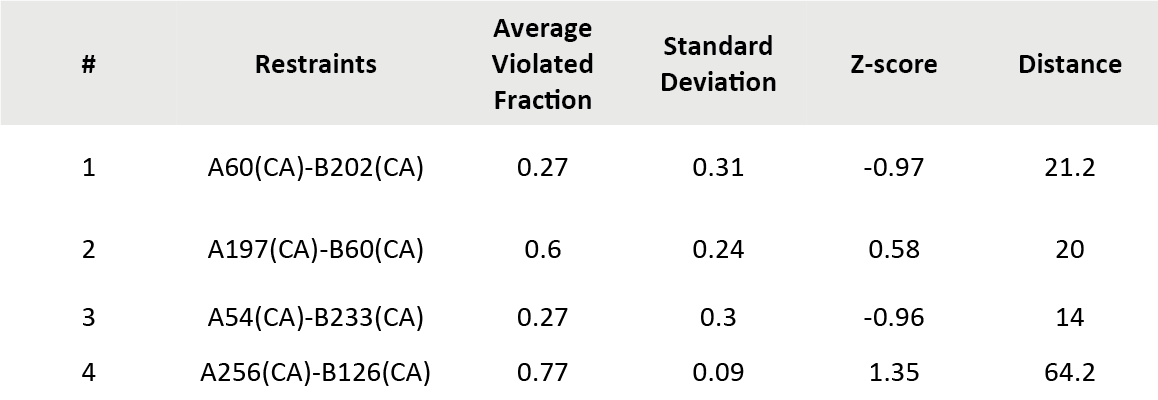
\includegraphics[]{Chapter.2/Figures/ts3.png}
    \captionsetup{singlelinecheck = false, format= hang}
    \caption{
      \textbf{DisVis output example for potentially intersubunit Alpha-Enolase crosslinks.}
    }
    \label{tab:tabs2.3}
  \end{table*}
\end{subappendices}

\clearpage
\section*{References}
\bibliographystyle{Stylesettings/pnas}
\patchcmd{\thebibliography}
{\clubpenalty 4000\widowpenalty 4000}
{\clubpenalties 1 10000 \widowpenalties 1 10000}
{}{}
\bibliography{chapmerge}
\stopthumb

